\documentclass[a4paper]{article}

\usepackage[english]{babel}
\usepackage[utf8]{inputenc}
\usepackage{amsmath}
\usepackage{graphicx}
\usepackage[breaklinks]{hyperref}
\usepackage{caption}

\title{
	Project 02 \\
	\bigskip
	\normalsize APSC 607 Fall 2017
}

\author{Seth Goodman}

\date{\today}

\begin{document}
\maketitle


%\begin{abstract}
%\end{abstract}

\section{Introduction}
\label{sec:introduction}


This project explored methods for calculating the integral roots of functions. Each functions was  examined in the range between zero and two, using the Composite Trapezoidal Rule, Composite Midpoint Rule, Composite Simpson’s Rule, as well as an adaptive implementation of the Composite Simpson’s Rule. The behavior and characteristics of these methods are reviewed by examining the effectiveness of the resulting value for the integral given a range of values for N. 

All computations were performed using MATLAB using the code (Table 1) accompanying this report (in a zip file). The following Methods section will present the methods used in MATLAB to explore functions, as well as the outputs and results. The Results section of this report contains the outputs for each function and range along with related observations and discussion. All figures and tables found in this report are available in the output subdirectory of the accompanying zip file. Additionally, all code and figures found in the zip file can be accessed via GitHub\footnote{\url{https://github.com/sgoodm/apsc607/tree/master/project_02}}.



\newpage
\section{Test}

\LaTeX{} is great at typesetting mathematics. Let $X_1, X_2, \ldots, X_n$ be a sequence of independent and identically distributed random variables with $\text{E}[X_i] = \mu$ and $\text{Var}[X_i] = \sigma^2 < \infty$, and let


\begin{equation}
S_n = \frac{X_1 + X_2 + \cdots + X_n}{n}
      = \frac{1}{n}\sum_{i}^{n} X_i
\label{eq:sn}
\end{equation}

denote their mean. Then as $n$ approaches infinity, the random variables $\sqrt{n}(S_n - \mu)$ converge in distribution to a normal $\mathcal{N}(0, \sigma^2)$.

Use the table and tabular commands for basic tables --- see Table~\ref{tab:widgets}, for example.

\begin{table}
\centering
\begin{tabular}{l|r}
Item & Quantity \\\hline
Widgets & 42 \\
Gadgets & 13
\end{tabular}
\caption{\label{tab:widgets}An example table.}
\end{table}

You can make lists with automatic numbering \dots

\begin{enumerate}
\item Like this,
\item and like this.
\end{enumerate}
\dots or bullet points \dots
\begin{itemize}
\item Like this,
\item and like this.
\end{itemize}
\dots or with words and descriptions \dots
\begin{description}
\item[Word] Definition
\item[Concept] Explanation
\item[Idea] Text
\end{description}

Some text\cite{burden2010}.

\begin{equation}
f(x) = e^{2x} * sin(3x)
\label{eq:fa}
\end{equation}

\begin{equation}
f(x) = \frac{1}{x+4}
\label{eq:fb}
\end{equation}

here is ref to \ref{eq:fb}


before figure 1a
\begin{center}
	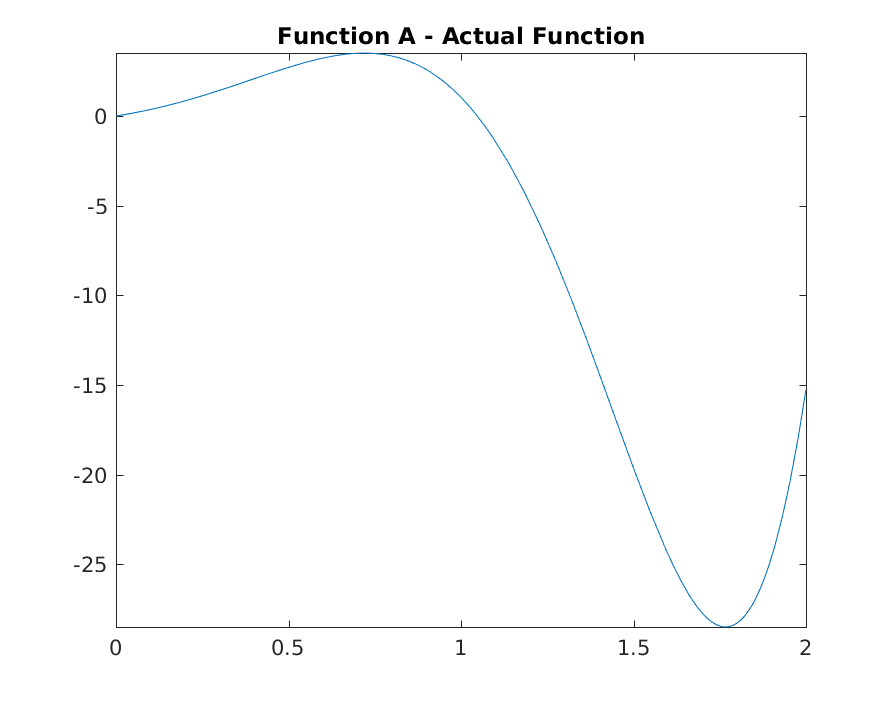
\includegraphics[width=1\textwidth]{../output/a_actual.png}
	\captionof{figure}{caption text a}
	\label{fig:figa}
\end{center}
after figure 1a



Figure \ref{fig:figa}\\



cool $B=0$ stuff 




sdsadas\footnote{See following link on MATLAB precision limitions (general limitations of floating point representations apply) https://www.mathworks.com/help/fixedpoint/ug/limitations-on-precision.html}


\newpage
\section{Methods}
\label{sec:methods}

\subsection{Trapezoidal}
TEXT


\subsection{Midpoint}
TEXT? 

\subsection{Simpson's}
TEXT

\subsection{Adaptive Simpson's}
TEST



\newpage
\section{Results}
\label{sec:results}

\subsection{Tables}
stuff



\newpage
\begin{thebibliography}{9}
\bibitem{burden2010}
  Burden, R., Faires, J., Numerical Analysis 9th Edition. 2010

\end{thebibliography}
\end{document}
